% Created 2014-04-03 Thu 21:46
\documentclass[table,smaller]{beamer}
\usepackage[utf8]{inputenc}
\usepackage[T1]{fontenc}
\usepackage{fixltx2e}
\usepackage{graphicx}
\usepackage{longtable}
\usepackage{float}
\usepackage{wrapfig}
\usepackage{rotating}
\usepackage[normalem]{ulem}
\usepackage{amsmath}
\usepackage{textcomp}
\usepackage{marvosym}
\usepackage{wasysym}
\usepackage{amssymb}
\usepackage{hyperref}
\tolerance=1000
\usepackage{tikz}
\usepackage{minted}
\usepackage{fancyvrb}
\usemintedstyle{perldoc}
\definecolor{lightgray}{gray}{0.96}
\setlength{\tabcolsep}{1ex}
\institute{Harvard MIT Data Center}
\usetheme{Warsaw}
\useoutertheme{infolines}
\setbeamercolor{block body}{bg=lightgray}
\titlegraphic{
\includegraphics[width=.75\textwidth]{images/IQSSNewLogo.pdf}}
\setbeamersize{text margin left=2em,text margin right=2em}
\AtBeginSection[]{\begin{frame}<beamer>\frametitle{Topic}\tableofcontents[currentsection]\end{frame}}
\usetheme{default}
\author{}
\date{}
\title{Stata Graphics}
\hypersetup{
  pdfkeywords={},
  pdfsubject={},
  pdfcreator={Emacs 24.3.1 (Org mode 8.2.5h)}}
\begin{document}

\maketitle
\begin{frame}{Outline}
\tableofcontents
\end{frame}


\section{Introduction}
\label{sec-1}
\rowcolors{1}{blue!15}{blue!3}
\definecolor{bg}{rgb}{0.95,0.95,0.95}
\definecolor{cbg}{cmyk}{0,0,.1,0}

\begin{frame}[fragile,label=sec-1-1]{Download workshop materials}
 \begin{itemize}
\item Download materials from \url{http://j.mp/stata-graph}
\item Extract materials from the \texttt{StataGraphics.zip} file
\item Launch Stata and open the \texttt{StataGraphics.do} file
\end{itemize}
\end{frame}

\begin{frame}[fragile,label=sec-1-2]{Organization}
 \begin{itemize}
\item Please feel free to ask questions at any point if they are relevant to the current topic (or if you are lost!)
\item There will be a Q\&A after class for more specific, personalized questions
\item Collaboration with your neighbors is encouraged
\item If you are using a laptop, you will need to adjust paths accordingly
\item Make comments in your Do-file rather than on hand-outs
\item Save on flash drive or email to yourself
\end{itemize}


\begin{block}{Graphing Strategies}
\begin{itemize}
\item Keep it simple
\item Labels, labels, labels!!
\item Avoid cluttered graphs
\item Every part of the graph should be meaningful
\item Avoid:
\begin{itemize}
\item Shading
\item Distracting colors
\item Decoration
\end{itemize}

\item Always know what you’re working with before you get started
\begin{itemize}
\item Recognize scale of data
\item If you’re using multiple variables – how do their scales align?
\end{itemize}
\item Before any graphing procedure review variables with \texttt{codebook}, \texttt{sum}, \texttt{tab}, etc.
\item HELPFUL STATA HINT:  If you want your command to go on multiple lines use \texttt{///} at end of each line
\end{itemize}
\end{block}

\begin{block}{Terrible Graph}
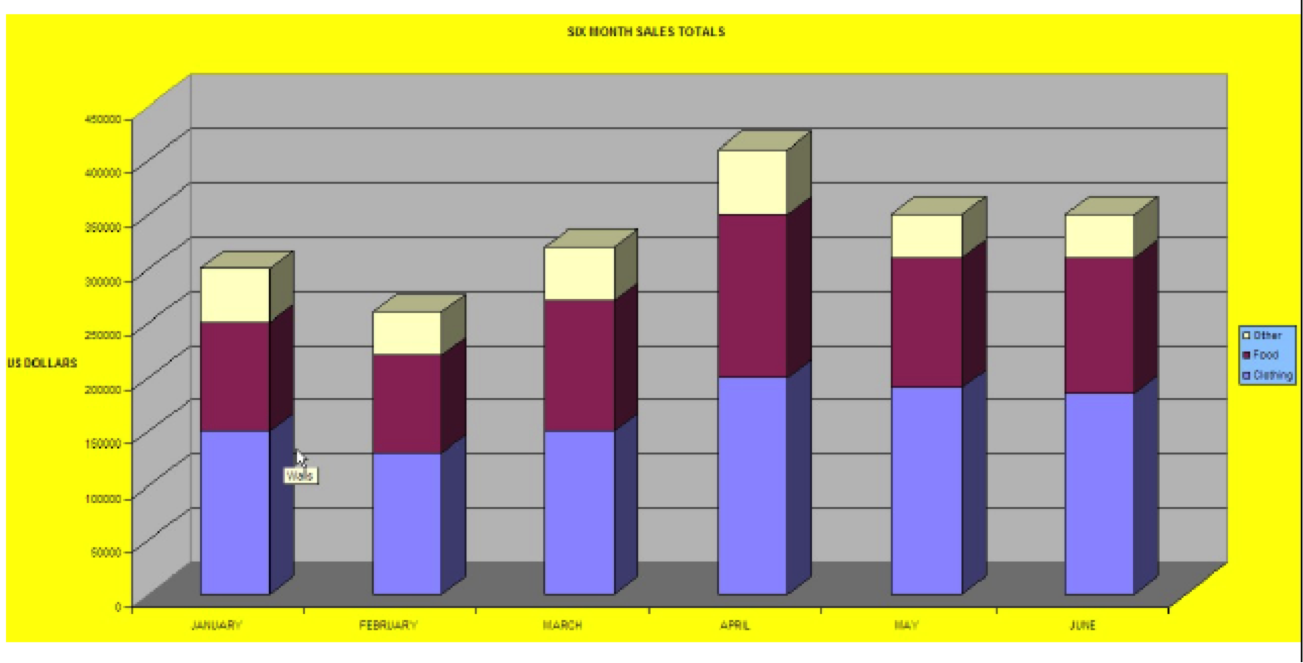
\includegraphics[width=.9\linewidth]{./images/Terrible.png}
\end{block}
\begin{block}{Much Better Graph}
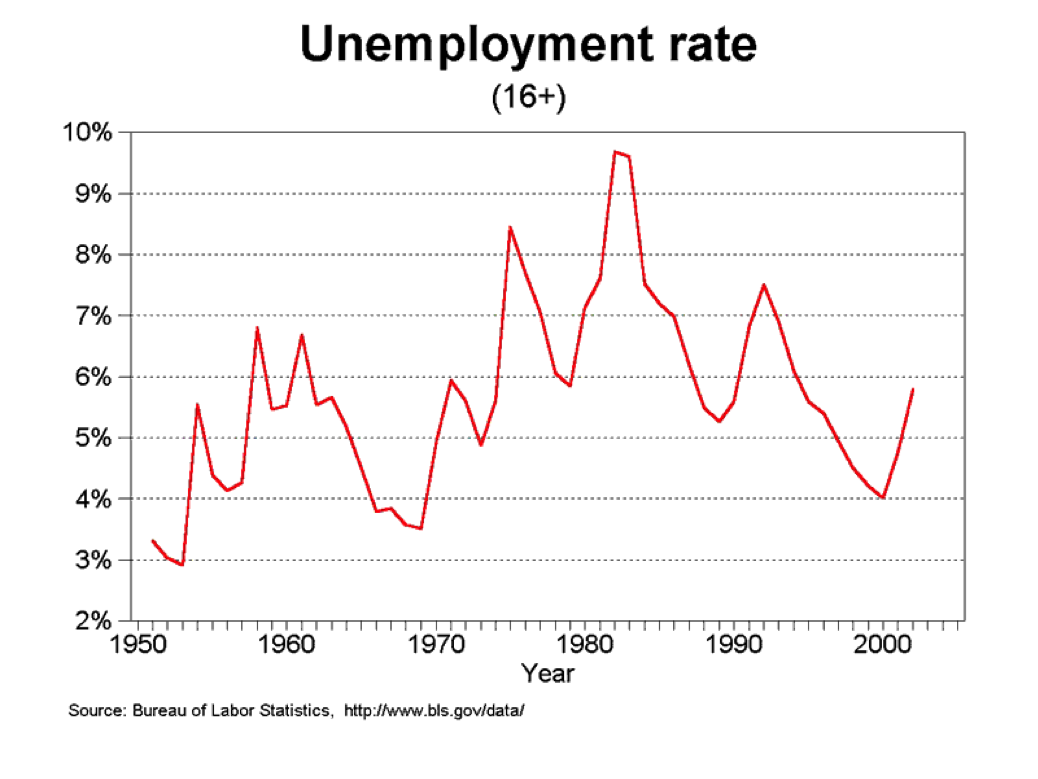
\includegraphics[width=.9\linewidth]{./images/Good.png}
\end{block}
\end{frame}



\section{Univariate Graphics}
\label{sec-2}

\begin{frame}[fragile,label=sec-2-1]{Our First Dataset}
 \begin{itemize}
\item Time Magazine Public School Poll
\begin{itemize}
\item Based on survey of 1,000 adults in U.S.
\item Conducted in August 2010
\item Questions regarding feelings about parental involvement, teachers union, current potential for reform
\end{itemize}

\item Open Stata and call up the datafile for today
\end{itemize}

\vspace{-.5em} \begin{columns} \column{.85\linewidth} \begin{block}{}
\begin{minted}[fontsize=\footnotesize]{c}
// Step 1: tell Stata where to find data:
cd /Users/dataclass/Desktop/StataGraphics/dataSets
// Step 2: call up our dataset:
use TimePollPubSchools.dta
\end{minted}
\end{block} \end{columns}
\end{frame}

\begin{frame}[fragile,label=sec-2-2]{Single Continuous Variables}
 Example: Histograms
\begin{itemize}
\item Stata assumes you’re working with continuous data
\item Very simple syntax: 
\begin{itemize}
\item \texttt{hist varname}
\end{itemize}
\item Put a comma after your varname and start adding options
\begin{itemize}
\item \texttt{bin(\#)} : change the number of bars that the graph displays
\item \texttt{normal} : overlay normal curve
\item \texttt{addlabels} : add actual values to bars
\end{itemize}
\end{itemize}
\end{frame}

\begin{frame}[fragile,label=sec-2-3]{Histogram Options}
 \begin{itemize}
\item To change the numeric depiction of your data add these options after the comma 
\begin{itemize}
\item Choose one: density fraction frequency percent
\end{itemize}
\item Be sure to properly describe your histogram:
\begin{itemize}
\item \texttt{title(insert name of graph)}
\item \texttt{subtitle(insert subtitle of graph)}
\item \texttt{note(insert note to appear at bottom of graph)}
\item \texttt{caption(insert caption to appear below notes)}
\end{itemize}
\end{itemize}
\end{frame}
\begin{frame}[fragile,label=sec-2-4]{Histogram Example}
 \vspace{-.5em} \begin{columns} \column{.85\linewidth} \begin{block}{}
\begin{minted}[fontsize=\footnotesize]{c}
hist F1, bin(10) percent title(TITLE) ///
  subtitle(SUBTITLE) caption(CAPTION) note(NOTES)
\end{minted}

\vspace{-1.5em}

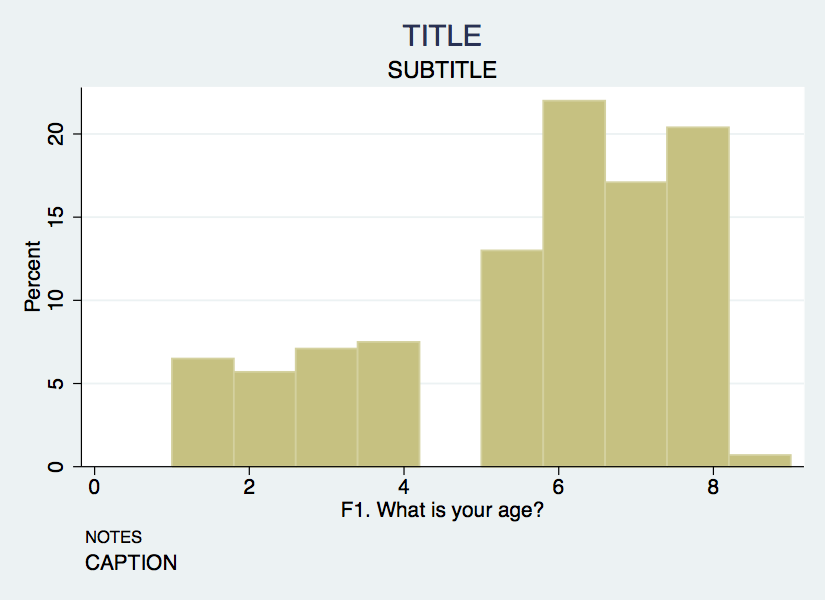
\includegraphics[width=.9\linewidth]{./images/hist1.png}

\end{block} \end{columns}
\end{frame}
\begin{frame}[fragile,label=sec-2-5]{Axis Titles and Labels}
 Example: Histograms
\begin{itemize}
\item Axis title options (default is variable label):
\begin{itemize}
\item \texttt{xtitle(insert x axis name)}
\item \texttt{ytitle(insert y axis name)}
\end{itemize}
\item Don’t want axis titles?
\begin{itemize}
\item \texttt{xtitle("")}
\item \texttt{ytitle("")}
\end{itemize}

\item Add labels to X or Y axis:
\begin{itemize}
\item xlabel(insert x axis label)
\item ylabel(insert y axis label)
\end{itemize}
\item Tell Stata how to scale each axis
\begin{itemize}
\item xlabel(start\#(increment)end\#)
\item xlabel(0(5)100)
\end{itemize}
\item This would label x-axis from 0-100 in increments of 5
\end{itemize}
\end{frame}
\begin{frame}[fragile,label=sec-2-6]{Axis Labels Example}
 \vspace{-.5em} \begin{columns} \column{.85\linewidth} \begin{block}{}
\begin{minted}[fontsize=\footnotesize]{c}
hist F1, bin(10) percent title(TITLE) subtitle(SUBTITLE) ///
    caption(CAPTION) note(NOTES) ///
    xtitle(Here's your x-axis title) ///
ytitle(here's your y-axis title)
\end{minted}

\vspace{-1.5em}

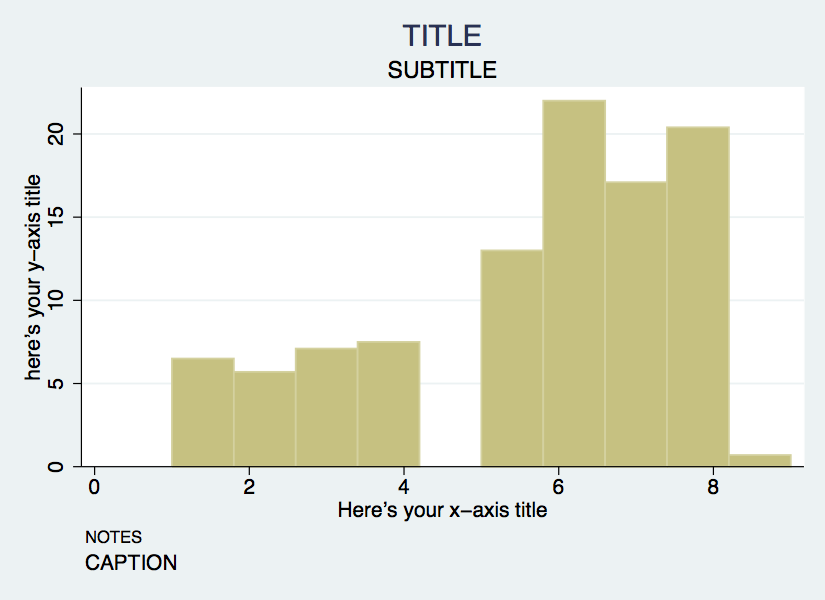
\includegraphics[width=.9\linewidth]{./images/hist2.png}

\end{block} \end{columns}
\end{frame}

\begin{frame}[fragile,label=sec-2-7]{Basic Graphing: Single Categorical Variables}
 \begin{itemize}
\item We can also use the \texttt{hist} command for bar graphs
\begin{itemize}
\item Simply specify "discrete" with options
\end{itemize}
\item Stata will produce one bar for each level (i.e. category) of variable
\item Use \texttt{xlabel} command to insert names of individual categories
\end{itemize}


\vspace{-.5em} \begin{columns} \column{.85\linewidth} \begin{block}{}
\begin{minted}[fontsize=\footnotesize]{c}
hist F4, title(Racial breakdown of Time Poll Sample) xtitle(Race) ///
ytitle(Percent) xlabel(1 "White" 2 "Black" 3 "Asian" 4 "Hispanic" ///
 5 "Other") discrete percent addlabels
\end{minted}

\vspace{-1.5em}

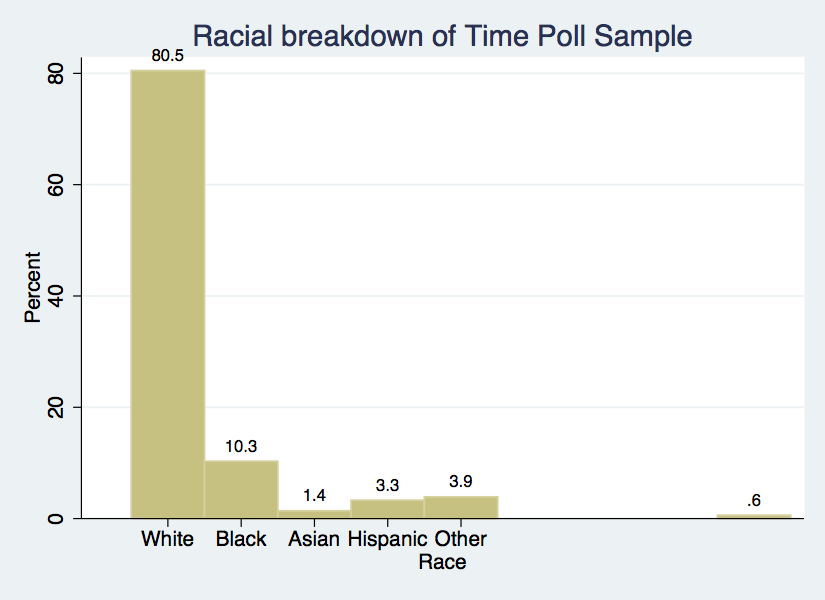
\includegraphics[width=.9\linewidth]{./images/bargraph.png}

\end{block} \end{columns}
\end{frame}

\begin{frame}[fragile,label=sec-2-8]{Exercise 1: Histograms Bar Graphs}
 \begin{enumerate}
\item Open the datafile, NatNeighCrimeStudy.dta.
\item Create a histogram of the tract-level poverty rate (variable name: \texttt{T\_POVRTY}).
\item Insert the normal curve over the histogram
\item Change the numeric representation on the Y-axis to "percent"
\item Add appropriate titles to the overall graph and the x axis and y axis.  Also, add a note that states the source of this data.
\item Open the datafile, TimePollPubSchools.dta
\item Create  a histogram of the question, "What grade would you give your child’s school" (variable name: Q11).  Be sure to tell Stata that this is a categorical variable.
\item Format this graph so that the axes have proper titles and labels.  Also, add an appropriate title to the overall graph that goes onto two lines.  Add a note stating the source of the data.
\end{enumerate}
\end{frame}

\begin{frame}[label=sec-2-9]{Next Dataset:}
\begin{itemize}
\item National  Neighborhood Crime Study (NNCS)
\begin{itemize}
\item N=9,593 census tracts in 2000
\item Explore sources of variation in crime for communities in the United States
\item Tract-level data: crime, social disorganization, disadvantage, socioeconomic inequality
\item City-level data: labor market, socioeconomic inequality, population change
\end{itemize}
\end{itemize}
\end{frame}

\section{Bivariate Graphics}
\label{sec-3}

\begin{frame}[fragile,label=sec-3-1]{The Twoway Family}
 \begin{itemize}
\item \texttt{twoway} is basic Stata command for all twoway graphs
\item Use \texttt{twoway} anytime you want to make comparisons among variables
\item Can be used to combine graphs (i.e., overlay one graph with another
\begin{itemize}
\item e.g., insert line of best fit over a scatter plot
\end{itemize}

\item Some basic examples:
\end{itemize}
\vspace{-.5em} \begin{columns} \column{.85\linewidth} \begin{block}{}
\begin{minted}[fontsize=\footnotesize]{c}
use NatNeighCrimeStudy.dta
twoway scatter T_PERCAP T_VIOLNT
twoway dropline T_PERCAP T_VIOLNT
twoway  lfitci T_PERCAP T_VIOLNT
\end{minted}
\end{block} \end{columns}
\end{frame}
\begin{frame}[fragile,label=sec-3-2]{Twoway and the "by" Statement}
 \vspace{-.5em} \begin{columns} \column{.85\linewidth} \begin{block}{}
\begin{minted}[fontsize=\footnotesize]{c}
twoway scatter T_PERCAP T_VIOLNT, by(DIVISION)
\end{minted}



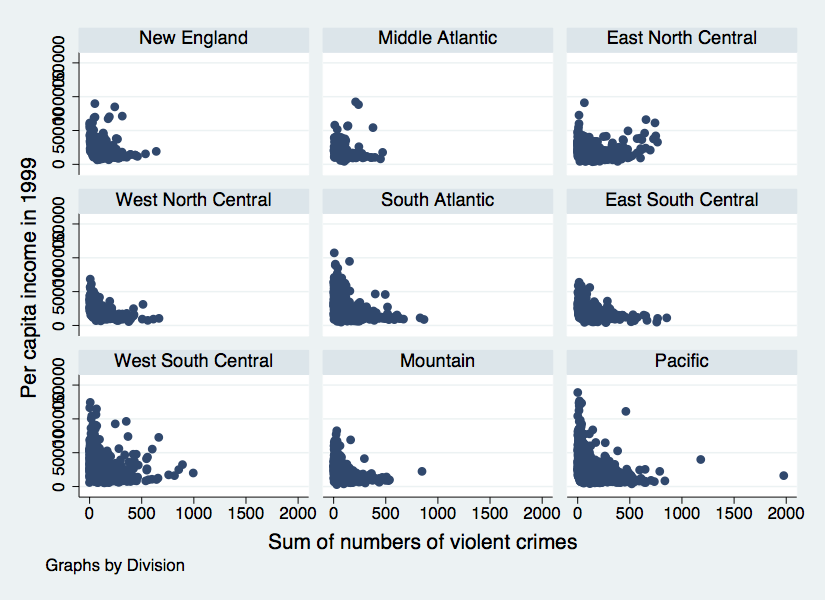
\includegraphics[width=.9\linewidth]{./images/twowayby.png}

\end{block} \end{columns}
\end{frame}

\begin{frame}[fragile,label=sec-3-3]{Twoway Title Options}
 \begin{itemize}
\item Same title options as with histogram
\begin{itemize}
\item \texttt{title(insert name of graph)}
\item \texttt{subtitle(insert subtitle of graph)}
\item \texttt{note(insert note to appear at bottom of graph)}
\item \texttt{caption(insert caption to appear below notes)}
\end{itemize}
\end{itemize}
\end{frame}
\begin{frame}[fragile,label=sec-3-4]{Twoway Title Options Example}
 \vspace{-.5em} \begin{columns} \column{.85\linewidth} \begin{block}{}
\begin{minted}[fontsize=\footnotesize]{c}
twoway scatter T_PERCAP T_VIOLNT, ///
    title(Comparison of Per Capita Income ///
	  and Violent Crime Rate at Tract level) ///
xtitle(Violent Crime Rate) ytitle(Per Capita Income) ///
    note(Source: National Neighborhood Crime Study 2000)
\end{minted}

\end{block} \end{columns}

\begin{itemize}
\item The title is a bit cramped--let's fix that:
\end{itemize}

\vspace{-.5em} \begin{columns} \column{.85\linewidth} \begin{block}{}
\begin{minted}[fontsize=\footnotesize]{c}
twoway scatter T_PERCAP T_VIOLNT, ///
    title("Comparison of Per Capita Income" ///
"and Violent Crime Rate at Tract level") ///
xtitle(Violent Crime Rate) ytitle(Per Capita Income) ///
note(Source: National Neighborhood Crime Study 2000)
\end{minted}

\end{block} \end{columns}
\end{frame}

\begin{frame}[fragile,label=sec-3-5]{Twoway Symbol Options}
 \begin{itemize}
\item A variety of symbol shapes are available: use \texttt{palette symbolpalette} to seem them and \texttt{msymbol()} to set them
\end{itemize}
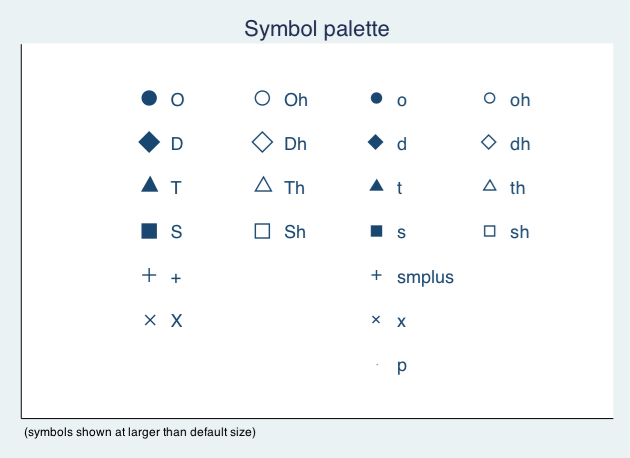
\includegraphics[width=.9\linewidth]{./images/Symbol.png}
\end{frame}
\begin{frame}[fragile,label=sec-3-6]{Twoway Symbol Options}
 \vspace{-.5em} \begin{columns} \column{.85\linewidth} \begin{block}{}
\begin{minted}[fontsize=\footnotesize]{c}
twoway scatter T_PERCAP T_VIOLNT, ///
    title("Comparison of Per Capita Income" ///
"and Violent Crime Rate at Tract level") ///
xtitle(Violent Crime Rate) ytitle(Per Capita Income) ///
note(Source: National Neighborhood Crime Study 2000) ///
msymbol(Sh) mcolor("red")
\end{minted}

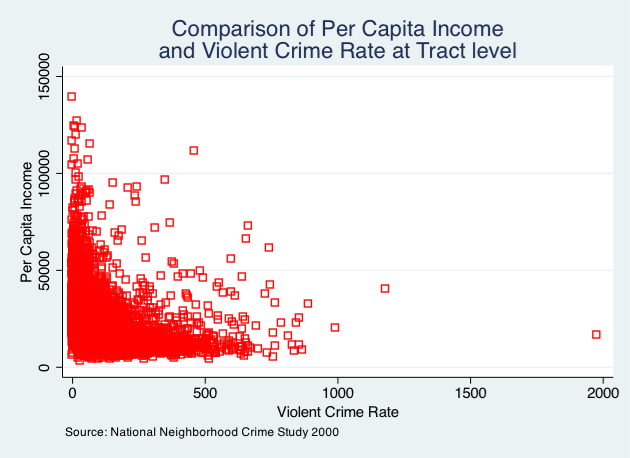
\includegraphics[width=.9\linewidth]{./images/msymbol_mcolor.png}

\end{block} \end{columns}
\end{frame}


\begin{frame}[fragile,label=sec-3-7]{Overlaying Twoway Graphs}
 \begin{itemize}
\item Very simple to combine multiple graphs…just put each graph command in parentheses
\begin{itemize}
\item \texttt{twoway (scatter var1 var2) (lfit var1 var2)}
\end{itemize}
\item Add individual options to each graph within the parentheses
\item Add overall graph options as usual following the comma 
\begin{itemize}
\item \texttt{twoway (scatter var1 var2) (lfit var1 var2), options}
\end{itemize}
\end{itemize}
\end{frame}
\begin{frame}[fragile,label=sec-3-8]{Overlaying Points and Lines}
 \vspace{-.5em} \begin{columns} \column{.85\linewidth} \begin{block}{}
\begin{minted}[fontsize=\footnotesize]{c}
twoway (scatter T_PERCAP T_VIOLNT) ///
    (lfit T_PERCAP T_VIOLNT), ///
    title("Comparison of Per Capita Income" ///
	  "and Violent Crime Rate at Tract level") ///
    xtitle(Violent Crime Rate) ytitle(Per Capita Income) ///
    note(Source: National  Neighborhood Crime Study 2000)
\end{minted}

\end{block} \end{columns}
\end{frame}
\begin{frame}[fragile,label=sec-3-9]{Overlaying Points and Labels}
 \vspace{-.5em} \begin{columns} \column{.85\linewidth} \begin{block}{}
\begin{minted}[fontsize=\footnotesize]{c}
twoway (scatter T_PERCAP T_VIOLNT if T_VIOLNT==1976, ///
	mlabel(CITY)) (scatter T_PERCAP T_VIOLNT), ///
    title("Comparison of Per Capita Income" ///
	  "and Violent Crime Rate at Tract level") ///
    xlabel(0(200)2400) note(Source: National Neighborhood ///
			    Crime Study 2000) legend(off)
\end{minted}

\end{block} \end{columns}
\end{frame}

\begin{frame}[fragile,label=sec-3-10]{Exercise 2: The TwoWay Family}
 Open the datafile, NatNeighCrimeStudy.dta.
\begin{enumerate}
\item Create a basic twoway scatterplot that compares the city unemployment rate (\texttt{C\_UNEMP}) to the percent secondary sector low-wage jobs (\texttt{C\_SSLOW})
\item Generate the same scatterplot, but this time, divide the plot by the dummy variable indicating whether the city is located in the south or not (\texttt{C\_SOUTH})
\item Change the color of the symbol that you use in this scatter plot
\item Change the type of symbol you use to a marker of your choice
\item Notice in your scatterplot that is broken down by \texttt{C\_SOUTH}  that there is an outlier in the upper right hand corner of the "Not South" graph.  Add the city name label to this marker.
\item Review the options available under "help twoway$_{\text{options}}$" and change one aspect of your graph using an option that we haven’t already reviewed
\end{enumerate}
\end{frame}

\section{More Fun with Twoway Line Graphs}
\label{sec-4}

\begin{frame}[fragile,label=sec-4-1]{Line Graphs}
 \begin{itemize}
\item Line graphs helpful for a variety of data
\begin{itemize}
\item Especially any type of time series data
\end{itemize}
\item We’ll use data on US life expectancy from 1900-1999
\begin{itemize}
\item \texttt{webuse uslifeexp, clear}
\end{itemize}
\end{itemize}
\end{frame}
\begin{frame}[fragile,label=sec-4-2]{Line Graphs}
 \vspace{-.5em} \begin{columns} \column{.85\linewidth} \begin{block}{}
\begin{minted}[fontsize=\footnotesize]{c}
webuse uslifeexp, clear
twoway (line le_wm year, mcolor("red")) ///
    (line le_bm year, mcolor("green"))
\end{minted}

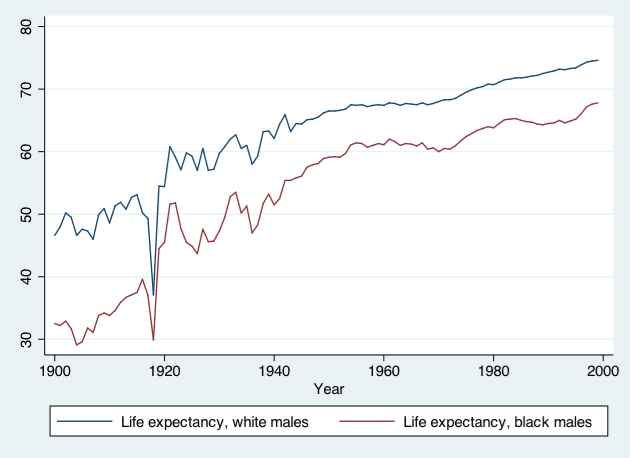
\includegraphics[width=.9\linewidth]{./images/lineGraph1.png}

\end{block} \end{columns}
\end{frame}

\begin{frame}[fragile,label=sec-4-3]{Line Graphs}
 \vspace{-.5em} \begin{columns} \column{.85\linewidth} \begin{block}{}
\begin{minted}[fontsize=\footnotesize]{c}
twoway (line (le_wfemale le_wmale le_bf le_bm) year, ///
    lpattern(dot solid dot solid))
\end{minted}

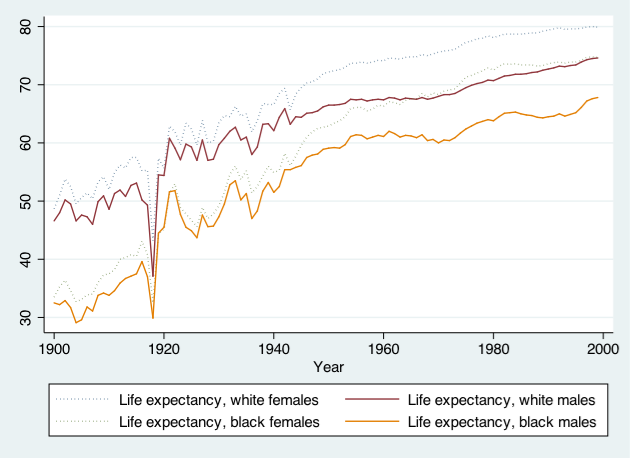
\includegraphics[width=.9\linewidth]{./images/linegraph2.png}

\end{block} \end{columns}
\end{frame}

\begin{frame}[fragile,label=sec-4-4]{Stata Graphing Lines}
 \vspace{-.5em} \begin{columns} \column{.85\linewidth} \begin{block}{}
\begin{minted}[fontsize=\footnotesize]{c}
palette linepalette
\end{minted}

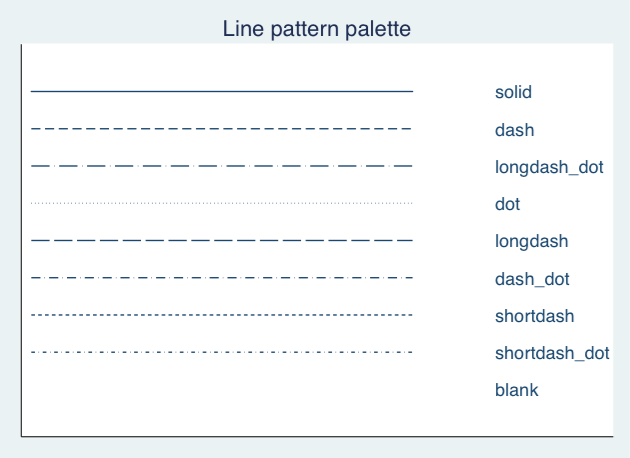
\includegraphics[width=.9\linewidth]{./images/linepalette.png}

\end{block} \end{columns}
\end{frame}

\begin{frame}[fragile,label=sec-4-5]{Exporting Graphs}
 \begin{itemize}
\item From Stata, right click on image and select "save as" or try syntax:
\begin{itemize}
\item \texttt{graph export myfig.esp, replace}
\end{itemize}
\item In Microsoft Word: insert > picture > from file
\begin{itemize}
\item Or, right click on graph in Stata and copy and paste into Word
\end{itemize}
\end{itemize}
\end{frame}


\section{Wrap-up}
\label{sec-5}

\begin{frame}[label=sec-5-1]{Help Us Make This Workshop Better}
\begin{itemize}
\item Please take a moment to fill out a very short feedback form
\item These workshops exist for you--tell us what you need!
\item \url{http://tinyurl.com/StataGraphicsFeedback}
\end{itemize}
\end{frame}
\begin{frame}[label=sec-5-2]{Additional resources}
\begin{itemize}
\item training and consulting
\begin{itemize}
\item IQSS workshops: \url{http://projects.iq.harvard.edu/rtc/filter_by/workshops}
\item IQSS statistical consulting: \url{http://rtc.iq.harvard.edu}
\end{itemize}

\item Stata resources
\begin{itemize}
\item UCLA website: \url{http://www.ats.ucla.edu/stat/Stata/}
\item Great for self-study
\item Links to resources
\end{itemize}
\item Stata website: \url{http://www.stata.com/help.cgi?contents}
\item Email list: \url{http://www.stata.com/statalist/}
\end{itemize}
\end{frame}
% Emacs 24.3.1 (Org mode 8.2.5h)
\end{document}